% Requires in the preamble: \usepackage{graphicx} (already in the ACL template) and \usepackage{subcaption}
% Images: upload eacl-rebuttal/figures/stimuli/{train-sg,train-pl,dev-sg,dev-pl}.jpg to figures/stimuli/ in Overleaf.
\begin{figure*}[t]
    \centering
    \footnotesize
    % ---------------- Vision: training ----------------
    \begin{subfigure}[t]{0.48\textwidth}
        \centering
        \begin{tabular}{@{}cc@{}}
            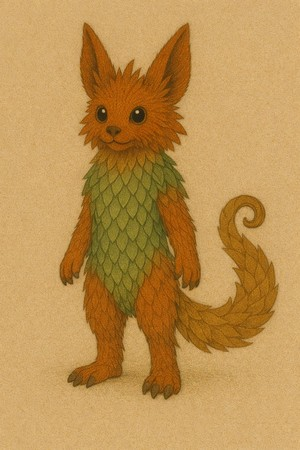
\includegraphics[height=0.95in]{figures/stimuli/train-sg.jpg} &
            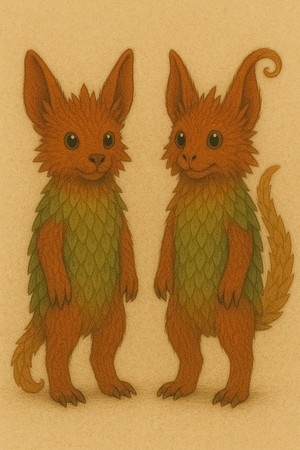
\includegraphics[height=0.95in]{figures/stimuli/train-pl.jpg} \\[2pt]
            \multicolumn{2}{c}{\textit{Caption this image.}} \\
            Look at the \texttt{[wug]}. & Look at the \texttt{[wugs]}.
        \end{tabular}
        \caption{Vision: training}
    \end{subfigure}\hfill
    % ---------------- Vision: development ----------------
    \begin{subfigure}[t]{0.48\textwidth}
        \centering
        \begin{tabular}{@{}cc@{}}
            
\includegraphics[height=0.95in]{figures/stimuli/dev-sg.jpg} &
            
\includegraphics[height=0.95in]{figures/stimuli/dev-pl.jpg} \\[2pt]
            \multicolumn{2}{c}{\textit{What do you see in this picture?}} \\
            I see the \underline{\hspace{1.2em}} $\rightarrow$ \texttt{[wug]} & I see the \underline{\hspace{1.2em}} $\rightarrow$ \texttt{[wugs]}
        \end{tabular}
        \caption{Vision: development}
    \end{subfigure}

    \vspace{8pt}

    % ---------------- Language: training ----------------
    \begin{subfigure}[t]{0.48\textwidth}
        \centering
        The \texttt{[wug]} shook its tail before running away.\\
        The \texttt{[wugs]} shook their tails before running away.
        \caption{Language: training}
    \end{subfigure}\hfill
    % ---------------- Language: development ----------------
    \begin{subfigure}[t]{0.48\textwidth}
        \centering
        The tiny \texttt{[wug]} \{jumps / *jump\}.\\
        The tiny \texttt{[wugs]} \{jump / *jumps\}.
        \caption{Language: development}
    \end{subfigure}

    \caption{Examples of training and development stimuli for \texttt{[wug]} and \texttt{[wugs]} in the vision (a--b) and language (c--d) cue conditions. In the vision condition, captions are identical for \texttt{[wug]} and \texttt{[wugs]}, and development items pair held-out images with prompts that end right before the novel noun. In (d), * marks the ungrammatical option.}
    \label{fig:stimuli}
\end{figure*}
